\chapter{Modello di Saint Venant}
	Il modello più semplice per studiare una trave è formulato da Saint Venant che, tramite delle opportune ipotesi semplificative, permette di facilitare la descrizione del problema.
	
	\figura{7}{0.7}{schemasaintvenant}{schema di riferimento della trave di Saint Venant}{schemasaintvenant}
	
	\begin{concetto}
		Il \textbf{solido di Saint Venant}, figura \ref{schemasaintvenant}, è descritto da una trave di lunghezza $L$ sull'asse congiungente gli estremi $A$ e $B$. La terna di riferimento per l'analisi è posta con $z$ coincidente all'asse della trave, mentre gli assi $x,y$ sono posti in modo da formare un \textbf{sistema baricentrico principale} (per cui $I_{xy} = S_x = S_y = 0$).
		
		Le \textbf{ipotesi semplificative} necessarie per utilizzare il modello sono:
		\begin{itemize}
			\item che la lunghezza $L$ dell'asse sia di molto maggiore delle lunghezze caratteristiche delle sezioni. La trave deve essere rettilinea (o con raggio di curvatura molto alto) e la sezione deve essere costante (o variare blandamente lungo l'asse) e sempre perpendicolare all'asse in ogni punto della trave;
			\item che il mantello $\Gamma$ sia scarico e che non siano presenti azioni di volume $\ov b$. L'unico carico esterno che può essere applicato deve essere posto in corrispondenza delle basi $A$ e $B$.
		\end{itemize}
	\end{concetto}

	In generale nota la distribuzione di azioni superficiali $\ov f_A$ su una base ($A$ in questo caso), è possibile creare un sistema staticamente equivalente di risultante $\ov R_A$ e momento $\ov M_A$ rispetto al sistema baricentrico della trave:
	\[ \ov R_A= \int_{\Omega_A} \ov f_A\, d\Omega \qquad \ov M_A = \int_{\Omega_A} \ov r \times \ov f_A\, d\Omega \]
	
	In condizioni statiche è inoltre necessario che la risultante delle forze sul corpo sia nulla, da cui l'equazione $\ov R_A + \ov R_B=  \ov 0$, mentre bilanciando il momento rispetto al polo $A$ si ricava che $\ov M_A + \ov M_B + \ov O_A\ov O_B \times \ov R_B = \ov 0$.
	
	\begin{concetto}
		Si definisce dunque il \textbf{postulato di Saint Venant} per il quale \textit{noto che sulle basi $A,B$ della trave la tensione interna coincide con quella applicata dalle forze distribuite $\ov f_A,\ov f_B$, ad una distanza paragonabile alla dimensione caratteristica massima della base lo stato di tensione non dipende più dalla distribuzione delle azioni $\ov f$, ma solamente dalla risultante delle forze $\ov R$ e dal momento risultante $\ov M$.} \\
		La distanza dalla base rispetto alla quale lo stato di tensione dipende solamente dalla risultante è chiamata \textbf{distanza di estinzione}; nella fascia compresa tra base e distanza di estinzione non vale dunque il modello di Saint Venant.
	\end{concetto}
	\begin{osservazione}
		La distanza di estinzione è tanto minore quanto più compatta è la sezione della trave stessa.
	\end{osservazione}

\section{Stato tensionale}
	Nel modello di Saint Venant è possibile considerare la trave come composta da delle fibre longitutinali (lungo l'asse $z$) che possono reagire solamente a sforzi normali $\sigma_{zz}$ e ad azioni tangenziali del tipo $\tau_{xz},\tau_{yz}$; le altre azioni infatti sarebbero attivate solamente in corrispondenza di azioni sul mantello, cosa che per ipotesi del modello è scaratata. 
	
	In generale il modello può essere accettato fintanto che $\sxx,\syy,\txy \ll \szz,\txz\tyz$ e dunque il \textbf{tensore di Cauchy} si riduce ad uno stato tensionale piano del tipo
	\begin{equation}
		\S = \begin{bmatrix} \label{eq:sv:tensorecauchy}
			0 & 0 & \txz \\ 0 & 0 & \tyz \\ \txz & \tyz & \szz
		\end{bmatrix} \qquad \Rightarrow \quad \ov \szz = \szz \vers k \quad \ov \tau = \tyz \vers i + \txz \vers j
	\end{equation}
	Come è possibile osservare ogni vettore di tensione può essere scomposto in una componente normale alle sezioni $\ov \szz$ e in una componente di tipo tangenziale $\ov \tau$.
	
	\begin{concetto}
		La \textbf{soluzione} del problema di Saint Venant si basa dunque sul determinare il \textbf{campo scalare} associato all'azione normale $\sigma_{zz}(x,y)$ e al \textbf{campo vettoriale} $\ov \tau(x,y)$ associato alle componenti tangenziali.
	\end{concetto}

	Per il postulato di Saint Venant è possibile osservare che le componenti da determinzare $\szz,\txz,\tyz$ (funzioni della posizione), oltre la distanza di estinzione, sono indipendente della azioni di superficie $\ov f$ ma dipendono solamente dalle risultanti delle forze $\ov R = \big(T_x,T_y,N\big)$ e dei momenti $\ov M = \big(M_x, M_y, M_z\big)$.
	
	\begin{concetto}
		Nelle fasce di validità del modello di Saint Venant è dunque possibile istituire un'\textbf{equivalenza statica} tra le azioni staticamente equivalenti $\ov R,\ov M$ e lo stato di tensione interno e dunque:
		\begin{equation} \label{eq:sv:equivstatica}
		\begin{split}
			T_x = \int_{\Omega_s} \txz(x,y)\, d\Omega_s  \qquad & T_y =  \int_{\Omega_s} \tyz(x,y)\, d\Omega_s \\
			N = \int_{\Omega_s} \szz(x,y)\, d\Omega_s \qquad & M_z = \int_{\Omega_s} \Big(x\, \tyz(x,y) - y\,\txz(x,y)\Big) \, d\Omega_s \\
			M_x = \int_{\Omega_s}y \, \szz(x,y)\, d\Omega_s \qquad & M_y = \int_{\Omega_s}x \, \szz(x,y)\, d\Omega_s \\
		\end{split}
		\end{equation}
	\end{concetto}
	\begin{osservazione}
		Osservando l'equivalenza statica nel modello di Saint Venant (eq. \ref{eq:sv:equivstatica}) è possibile osservarae come la reazione normale $N$ e i momenti flettenti $M_x,M_y$ siano associati solamente al campo scalare $\szz$, e dunque ad un tensore del tipo
		\[\S = \begin{bmatrix}
			0 & 0 & 0 \\ 0 & 0 & 0 \\ 0 & 0 & \szz
		\end{bmatrix}\]
		
		Al contrario il momento torcente $M_z$ è associato alla presenza delle componenti $\txz$ e $\tyz$ che, di conseguenza, generano delle azioni taglianti $T_x,T_y$; queste azioni di fatto determinano il tensore di Cauchy del tipo
		\[\S = \begin{bmatrix}
		0 & 0 & \txz \\ 0 & 0 & \tyz \\ \txz & \tyz & 0
		\end{bmatrix}\]
		
	\end{osservazione}
	
	\subsection{Equilibrio indefinito, condizioni al contorno e legame costitutivo}
		\paragraph{Equilibrio indefinito} Come visto nell'equazione \ref{eq:sv:tensorecauchy}, lo stato tensionale di una trave sotto le ipotesi di Saint Venant è piano; considerando che per ipotesi le azioni di volume sono nulle ($\ov b=\ov0$) allora è possibile riscrivere le \textbf{equazioni di equilibrio indefinito} per il problema come:
		\[ \pd \txz z = 0 \qquad \pd \tyz z = 0 \qquad \pd \txz x + \pd \tyz y + \pd \szz z = 0 \]
		Le prime due equazioni dimostrano dunque che le \textbf{componenti tangenziali} $\tau_{xz},\tyz$ del vettore $\ov \tau$ sono \textbf{indipendenti} dalla coordinata assiale $z$, mentre la terza equazione lega la divergenza del campo delle azioni di taglio con la variazione lungo l'asse si $\szz$:
		\[ \textrm{div} \big(\ov \tau \big) = - \pd \szz z \begin{cases}
			= 0 \qquad & \textrm{: campo solenoidale, linee di flusso chiuse} \\
			\neq 0 \qquad & \textrm{: campo non solenoidale, linee di flusso aperte} \\
		\end{cases} \]
	
		\paragraph{Condizioni al contorno} L'ipotesi di Saint Venant afferma che il mantello sia sempre scarico; scelto un qualsiasi punto sull contorno avente direzione normale uscente $\vers n_\Gamma = \big(\alpha_x,\alpha_y,0\big)$ al punto considerato sul mantello $\Gamma$, allora si deve verificare che lo stato di tensione in quel punto sia nullo:
		\[  \begin{bmatrix} 
			0 & 0 & \txz \\ 0 & 0 & \tyz \\ \txz & \tyz & \szz
		\end{bmatrix} \begin{pmatrix}
			\alpha_x \\ \alpha_y \\ 0 
		\end{pmatrix} = \begin{pmatrix}
			0 \\ 0 \\ 0
		\end{pmatrix} \qquad \Rightarrow\quad \txz \alpha_x + \tyz \alpha_y = \ov \tau \cdot \vers n_\Gamma = 0 \quad \Leftrightarrow \quad \ov \tau \perp \vers n_\Gamma \]
		Si osserva dunque che sul mantello il vettore delle tensioni tangenziali $\ov \tau$ deve necessariamente essere ortogonale alla normale del mantello $\vers n_\Gamma$ (e dunque deve essere tangente alla superficie del mantello $\Gamma$ stesso).
		
		\begin{nota}
			In questo caso il versore $\vers n_\Gamma$ presenta l'ultima componente nulla in quanto, per ipotesi, la sezione è costante lungo l'asse della trave, e dunque il mantello non può avere componente normale nell'asse $z$. In caso di variazioni blande della sezione si avrebbe l'introduzione di tale fattore, che tuttavia sarebbe approssimabile al valore nullo.
			
		\end{nota}
		
		\paragraph{Legame costitutivo} Considerando che lo stato di tensione della trave è piano con vettore di tensione $\ov \sigma= (0,0,\szz,\tyz,\txz,0)$, allora considerando la matrice di cedevolezza $\C$ del legame costitutivo elastico lineare per il quale
		\[ \exx = - \frac \nu E \szz \quad \eyy -\frac \nu E \szz \quad \varepsilon_{zz} = \frac \szz E \quad \gamma_{xz} = \frac \txz G \quad \gamma_{yz} = \frac \tyz G \quad \gamma_{xy} = 0  \]
		E' inoltre possibile ricavare la formulazione del potenziale elastico (e relativo complementare) $\phi$ e $\psi$ considerando le componenti di tensione presenti nella trave, e dunque
		\begin{align*}
			\phi = \psi & = \frac{\szz^2}{2E} + \frac{\txz^2}{2G} + \frac{\tyz^2}{2G} = \frac{\szz^2}{2E} + \frac{\tau^2}{2G} \\ 
			& = \frac E 2 \varepsilon_{zz}^2 + \frac G 2 \big(\gamma_{xz}^2 + \gamma_{yz}^2\big)
		\end{align*}
		
	\subsection{Estensione al modello di Saint Venant}
		Per quanto riguarda le \textbf{condizioni sull'asse} è possibile accettare come travi rettilinee tutte le trave il cui raggio di curvatura sia molto maggiore delle dimensioni caratteristiche della sezione; per quanto riguarda la \textbf{sezione} inoltre è possibile ammettere tutte le travi le cui sezioni variano molto blandamente (\textit{pendenza} locale del mantello di qualche grado). \\
		Nel caso in cui si abbiano brusche distorsioni dell'asse e delle sezioni è necessario utilizzare dei modelli più raffinati (o integrare dei coefficienti correttivi) e considerare una nuova distanza di estinzione rispetto all'intorno rispetto al quale il modello non è accettabile.
		
		\vspace{3mm}
		Per quanto riguarda le \textbf{condizioni di carico} è possibile considerare il modello come valido, in presenza di carichi distribuiti sul mantello, ogni qualvolta che 
		\[ \sxx,\syy,\txy \ll \szz,\txz\tyz  \]
		In questa situazione gli effetti di carico sul mantello vengono trascurati in quanto irrisori rispetto alle altre azioni; in caso di carichi concentrati, come nel caso della geometria variabile, è necessario utilizzare modelli più raffinati o coefficienti correttivi introducendo un'ulteriore distanza di estinzione.
		
\section{Soluzione generale nelle tensioni}
	Per risolvere il problema generale delle tensioni della trave secondo il modello di Saint Venant si utilizza un approccio semi-inverso per il quale si suppone una soluzione del problema e si verifica che la stessa sia coerente con le equazioni caratteristiche.
	
	\begin{concetto}
		In primo luogo è possibile studiare il campo scalare $\szz(x,y)$ associato all'azione normale $N$ e ai momenti flettenti $M_x,M_y$; in assenza di momento torcente $M_z$, il campo vettoriale $\ov \tau$ sarebbe nullo solamente se i momenti flettenti fossero costanti lungo il solido, in quanto
		\[ T_y = \frac{dM_x}{dz}=0 \qquad T_x = - \frac{dM_y}{dz} = 0 \]
	\end{concetto}		
	
	\paragraph{Ipotesi deformativa} Osservando la deformazione del concio elementare che costituisce la trave si è osservato che la sezione della trave risulta sempre essere perpendicolare all'asse della trave stesso. Per le considerazioni appena mostrate, le azioni di momento flettente sono supposte costanti lungo tutta la trave e dunque rappresentano un carico simmetrico per ogni concio elementare.
	
	\figura{7}{0.7}{deformazioneconcio}{deformazione del concio elementare soggetto a solo forza normale (sinistra) e solo momento flettente (destra).}{deformazioneconcio}
	
	\figura{7}{0.7}{assedeformato}{lungo l'asse della trave ogni sezione deve essere sempre perpendicolare all'asse stesso.}{assedeformato}
		
	\subsection{Campo di deformazione, di tensione ed energia potenziale}
		
		Per quanto riguarda il \textbf{campo di deformazione}, come si osserva in figura \ref{assedeformato}, si vuol far si che le sezioni siano sempre perpendicolari all'asse della trave.
		\begin{concetto}
			Questo ci permette di ipotizzare che il \textbf{campo di deformazione} $\varepsilon_{zz}$ sia costante o quanto meno lineare lungo gli assi $x,y$, assumendo dunque una formulazione del tipo
			\begin{equation} \label{eq:sv:ipotesideflin}
				\varepsilon_{zz} = ax + by + c
			\end{equation}
		\end{concetto}
		In questo modo è possibile ricondurre la sezione deformata all'equazione di un piano in coordinate $x,y$. Dalle ipotesi di simmetria del cacirco sul concio elementare è possibile asserire le seguenti relazioni per quanto riguarda le deformazioni angolari:
		\[ \gamma_{xz} = \gamma_{yz} = 0  \]
		
		Considerando invece lo \textbf{stato di tensione}, esso può essere analizzato con la legge di Hooke per la quale la tensione $\szz$ è legata alla deformazione $\varepsilon_{zz}$ in funzione del modulo di Young $E$ secondo la legge $ \szz = E\varepsilon_{zz} = E\big(ax + by + c\big)$; unendo a questo risultato le prime due equazioni di equilibrio si ottiene al deformazione lungo gli assi $x$ e $y$ come:
		\[ \Rightarrow \quad \exx = \eyy = - \frac \nu E \szz = - \nu \varepsilon_{zz} \]
		
		\begin{nota}
			In questo caso si sta discutendo il caso in cui si ha la presenza del solo campo scalare $\szz$, e non del campo vettoriale $\ov \tau$.
		\end{nota}
		Per ipotesi la tensione della trave $\szz$ deve essere costante lungo la sezione, e dunque la terza equazione di equilibrio si riduce all'espressione
		\[ \pd \szz z = 0 \]
		
		\paragraph{Equivalenza statica} Per ogni sezione di concio elementare nel modello di Saint Venant deve dunque insistere una relazione di equivalenza statica tra le azioni interne e lo stato di tensione del materiale; come ipotesi iniziale dell'analisi dello stato di tensione normale si erano considerati nulli i termini $T_x,T_y,M_z$ in quanto indipendenti da $\szz$. Al contrario è invece possibile stabilire l'equivalenza statica per l'azione normale e i momenti flettenti dipendenti dal campo scalare $\szz$ come segue:
		\begin{align*}
			N & = \int_A \sigma_{zz} \, dA = \int_A Eax\, dA + \int_A Eby \, dA + \int_A Ec\, dA \\
			& = \cancel{EaS_y} + \cancel{EbS_x} + EcA  \\
			M_x & \int_A \sigma_{zz} y \, dA = \int_A Eaxy\, dA + \int_A Eby^2 \, dA + \int_A Ecy\, dA \\
			& = \cancel{EaI_{xy}} + EbI_{xx}+ \cancel{EcS_x}  \\
			M_y & -\int_A \sigma_{zz} x \, dA = -\int_A Eax^2\, dA - \int_A Ebxy \, dA - \int_A Ecx\, dA \\
			& = -EaI_{yy} -\cancel{ EbI_{xy}}- \cancel{EcS_y}  
		\end{align*}
		\begin{nota}
			I termini $S_y,S_x,I_{xy}$ possono essere trascurati in quanto, come ipotesi iniziale, si era considerato il sistema di riferimento come baricentrico, e dunque tali contributi sono conseguentemente sempre nulli.
		\end{nota}
		
		\begin{concetto}
			Dalle relazioni appena riportate è dunque possibile stabilire analiticamente i coefficienti di linearità $a,b,c$ presenti in equazione \ref{eq:sv:ipotesideflin}; in particolare è possibile definire il \textbf{campo di tensione} e di \textbf{deformazione} nel caso di sola componente scalare $\szz$ di tensione come
			\begin{equation} \label{eq:sv:szznormale}
				\szz = \frac NA + \frac \Mx \Ixx y - \frac \My \Iyy x  \qquad \varepsilon_{zz} = \frac N{EA} + \frac \Mx {E\Ixx} y - \frac \My {E \Iyy} x
			\end{equation}
		\end{concetto}
	
		\paragraph{Energia di deformazione} A questo punto è anche possibile calcolare l'\textbf{energia di deformazione elastica} $U_e$ per un materiale elastico isotropo lineare; per questo materiale infatti è noto il  potenziale elastico $\phi$ e relativo complementare $\psi$ che, integrati sul volume, determinano l'energia elastica:
		\[ \phi = \psi = \frac 1 2 \frac {\szz^2}E = \frac 1 2 E \varepsilon_{zz}^2 \qquad \Rightarrow \quad U_e = \int_V \phi = \int_L \underbrace{\int_A \frac 1 2 \frac {\szz^2}E\, dA }_{dU_e/dz} \, dz \]
		
		Avendo verificato in precedenza che la tensione $\szz$ è indipendente dalla coordinata $z$ è necessario valutare l'integrale associato alla variazione di energia lungo l'asse $dU_e/dz$. Nota l'espressione della tensione (eq. \ref{eq:sv:szznormale}) è dunque possibile valutare tale contributo come
		\begin{equation}
		\begin{split}
			\frac{dU_e}{dz} & = \frac 1{2E} \int_A \left(  \frac NA + \frac \Mx \Ixx y - \frac \My \Iyy x \right)^2\, dA \\
			& \frac 1{2E} \int_A \left(\frac{N^2}{A^2} + \frac{\Mx^2}{\Ixx^2}y^2 + \frac{\My^2}{\Iyy^2}x^2 + \cancel{\textrm{altri termini}} \right)\, dA \\
			& = \frac1 {2E} \left( \frac{N^2}A + \frac{\Mx^2}\Ixx + \frac {\My^2}\Iyy \right)
		\end{split}
		\end{equation}
		\begin{nota}
			Sviluppando opportunamente il quadrato dei contributi di $\szz$ è possibile osservare che gli altri membri, indicati come \textit{altri termini}, si elidono per via delle simmetrie nella scelta del sistema di riferimento baricentrico.
		\end{nota}

\section{Analisi della tensione normale}
	Vigendo il principio della sovrapposizione degli effetti è possibile descrivere lo stato di tensione analizzando l'effetto che ogni azione interna ha sulla trave; partendo analizzando l\textbf{azione normale} $N$, per come visto in equazione \ref{eq:sv:szznormale}, il campo scalare di tensione e conseguentemente di deformazione associato a tale azione è descritto dalle equazioni
	\[ \szz = \frac NA  \qquad \ezz = \frac N {EA} \qquad \exx = \eyy = -\nu \ezz = -\nu \frac N{EA} \]  
	\begin{osservazione}
		I termini $\sxx, \syy, \txy,\txz,\tyz, \gamma_{xy},\gamma_{xz}, \gamma_{yz}$ sono tutti nulli per tutte le ipotesi fin'ora considerate sul modello di Saint Venant.
	\end{osservazione}
	\begin{concetto}		
		Per integrazione delle equazioni di congruenza (\textbf{RIFERIMENTI}) associate al \textbf{campo di spostamento} $\ov u = (u,v,w)$ è possibile determinare le componenti scalari $u,v,w$ in funzione delle coordinate $x,y,z$ dei punti della trave:
		\begin{equation}\label{eq:sv:camponormale}
			\ov u = \left\{ \begin{split}
				u &= -\nu \frac N {EA} x + u_0(y,z) \\
				v &= -\nu \frac N {EA} y + v_0(x,z) \\
				w &= \frac N {EA} z + w_0(x,y) \\
			\end{split} \right.
		\end{equation}
	\end{concetto}
	In questa formulazione i termini $\big(u_0,v_0,w_0\big)$ sono delle funzioni di moto rigido dipendenti solamente dalla scelta del sistema di riferimento per per quali le equazioni di congruenza devono valere $\asmat{\partial} \ov u_0 = \ov 0$.
	\begin{osservazione}
		Essendo il termine $w_0$ costante e dipendente dalla scelta del sistema di riferimento, allora in generale la componente $w$ del campo di spostamento (che è la componente più \textit{importante} da analizzare in quanto descrive la compressione/estensione della trave) può essere espressa come
		\[ w(z) = \frac N{EA}z + c \qquad c \in \mathds R \textrm{ costante}\]
	\end{osservazione}
	\begin{osservazione}
		Dall'equazione \ref{eq:sv:camponormale} è possibile affermare che per una materiale standard (rapporto di Poisson $\nu$ compreso tra $0$ ed $\frac 1 2$) sottoposto a trazione ($N> 0$) la sua sezione diminuisce ($\exx, \eyy < 0$), mentre al contrario se è sottoposto a compressione ($N<0$) la sua sezione si espande ($\exx,\eyy > 0$). 
	\end{osservazione}
	\begin{concetto}
		E' possibile osservare che la \textbf{trasformazione} associata all'azione normale $N$ è \textbf{omotetica}, ossia mantiene invariato l'angolo relativo tra due segmenti qualsiasi prima e dopo trasformazione.		
	\end{concetto}
	\begin{dimostrazione}
		Noto che il tensore delle deformazioni $\E$ presenta solamente contributi diagonali $\exx,\eyy,\ezz$, scelta una generica retta radiale all'asse $z$ della trave di direzione $\vers r= \big(\cos\theta,\sin\theta,0\big)$, allora la sua deformazione lungo tale asse assume valore
		\[ \varepsilon_{rr} = \big(\E \vers r\big) \cdot \vers r = \exx \cos^2\theta + \eyy\sin^2\theta = - \nu \frac N{EA} \] 
		Questo dimostra dunque che la deformazione radiale $\varepsilon_{rr}$ è costante nella trave ed è indipendente dall'orientazione $\theta$ della retta $\vers r$ che si considera.
	\end{dimostrazione}

	E' possibile calcolare inoltre la variazione di volume considerando che l'elongazione volumetrica $\varepsilon_v$ è data dalla somma dei contributi delle deformazioni principali $\exx + \eyy + \ezz$ che porta al risultato
	\[ \varepsilon_v = \frac N{EA} ( 1 -2\nu) \qquad \Rightarrow \quad \Delta V = \int_V \varepsilon_v \, dV = \frac{NV}{EA} \big(1-2\nu\big) = \frac {NL} E \big(1-2\nu\big) \]
	dove il risultato finale si ottiene considerando la trave di volume $V$ come rettilinea di lunghezza assiale $L$ e sezione costante di area $A$.
	
	\begin{osservazione}
		Per \textbf{materiali standard} (rapporto di Poisson compreso tra 0 e $\frac 1 2$) è possibile affermare che la variazione volumetrica $\Delta V$ è sempre positiva per campioni sottoposti a trazione, e dunque si parla di materiali \textbf{dilatanti}. Nel caso particolare in cui $\nu = \frac 1 2$ si osserva che $\Delta V = 0$: la \textbf{deformazione} in questo caso è dunque \textbf{plastica}.
	\end{osservazione}

	\subsection{Rigidezza elastica equivalente}
		Si consideri come esempio la barra rettilinea mostrata in figura \ref{travevincolata}.
		\figura{6}{1}{travevincolata}{trave di lunghezza $L$ vincolata ad un estremo e caricata con azione normale $N$ all'estremo opposto.}{travevincolata}
		
		In questa situazione \textit{standard} il la componente $w$ del campo di spostamento $\ov u$ della barra è coerentemente modellato dall'espressione $w(z) = \frac N{EA}z + c$. Dalla scelta del sistema di riferimento si osserva che all'incastro, coordinata $z=0$, si deve ipotizzare spostamento nullo ($w=0$): questo permette di determinare che la costante $c$ è nulla e il campo di spostamento vale
		\[ w(z) = \frac N{EA}z  \]
		La variazione di lunghezza $\Delta L$ della trave può essere calcolata semplicemente valutando il campo di spostamento valutato nell'estremo opposto della trave, e dunque
		\[ \Delta L = w(L) = \frac{N}{EA}L \]
		
		\begin{concetto}
			Si osserva che la \textbf{trave} è \textbf{modellata} come una \textbf{molla lineare}; considerando infatti che l'azione normale $N$ coincide con la forza $F$ applicata sulla molla, allora l'allungamento della molla $\Delta x$ (associato alla variazione di lunghezza $\Delta L$) dipende dalla forza secondo un coefficiente $k$ dalla relazione
			\begin{equation}
				F = k\, \Delta x \qquad \leftarrow \quad k = \frac {EA} L
			\end{equation}
			dove il coefficiente $k$ prende il nome di \textbf{rigidezza elastica equivalente} della trave.
		\end{concetto}
		Considerando la trave come una molla, allora essa può essere equiparata ad un'\textbf{accumulatore di energia potenziale}; infatti è possibile dimostrare che l'energia immagazzinata da una molla (e dunque dalla trave) sottoposta ad una forza $F$ e allungamento $\Delta x$ secondo la legge
		\begin{equation}
			U_e = \frac 1 2 F\, \Delta x = \frac 1 2 N \, \Delta L = \frac 1 2 N \frac N{EA}L  = \frac 1 2 \frac{N^2}{EA}L
		\end{equation}
		\begin{osservazione}
			Per il teorema di Clapeyron è possibile osservare la relazione tra il lavoro associato alle azioni esterne e il lavoro interno dovuto alla deformazione elastica.
		\end{osservazione}
	
	\subsection{Verifica e dimensionamento}
		Nel caso si prova di pura trazione/compressione monoassiale, allora la tensione equivalente (per tutti i criteri) coincide con la tensione $\szz$ del sistema, e in particolare
		\[ \sigma_{eq} = \szz = \frac NA \]
		Posta la tensione critica $\sigma_{cr}$ del materiale e il coefficiente di sicurezza $\phi$ per il problema in equazione, la \textbf{verifica} si effettua invertendo la relazione $\sigma_{eq} \leq \sigma_{amm} = \sigma_{cr}\phi$, ottenendo dunque il risultato
		\[ N \leq \frac{\sigma_{cr}}{\phi} A \]
		
		Al contrario il \textbf{dimensionamento} si basa sul determinare l'area $A$ minima a supportare la tensione ammissibile; per fare questo è sufficiente manipolare l'equazione precedente ottenendo il risultato
		\[ A \geq \frac{N\phi}{\sigma_{cr}	} \]
		
		Le operazioni di verifica e dimensionamento possono essere anche effettuate mediante rappresentazione dello stato di tensione monoassiale sul piano di Mohr, come si osserva in figura \ref{mohrnormcrit}.
		
		\figura{4}{2}{mohrnormcrit}{rappresentazione dello stato di tensione nel piano di Mohr; aumentando la componente di azione normale $N$ lo stato di tensione associato (semicerchio blu) si espande fino a sovrapporsi al cerchio rappresentativo dello stato di tensione ammissibile (in rosso). }{mohrnormcrit}
		
	\subsection{Estensioni di validità}
		\paragraph{Estensioni geometriche} A questo punto è possibile cercare di capire quando è possibile estendere la soluzione dell'azione normale alle travi che non rispettano le ipotesi iniziali di Saint Venant. In particolare analizzando le \textbf{variazioni di sezione è possibile affermare che}:
		\begin{itemize}
			\item se la sezione \textbf{varia con regolarità} blandamente lungo l'asse, allora non è necessario introdurre una distanza di estinzione; noto dunque il valore dell'area $A(z)$ funzione della coordinata della trave è possibile ipotizzare che anche lo stato tensionale $\szz$ dipenda da $z$ secondo l'espressione
			\[ \szz (z) = \frac N {A(z)} \]
			In questa situazione decadrebbe la condizione di mantello scarico (le tensioni $\szz$ sulle areole esterne della sezione di fatto esercitano una forza sul mantello), tuttavia l'ipotesi di variazione blanda della sezione rende trascurabile tale effetto;
			
			\item se la sezione \textbf{varia bruscamente} è possibile utilizzare il modello di Saint Venant introducendo delle nuove  zone di estinzione e utilizzando le equazioni negli spezzoni di trave al di fuori delle stesse, come si può osservare in figura \ref{bruscvar}. In generale i 3 spezzoni ricavati possono avere anche proprietà del materiale diverse (quale il modulo elastico $E$). In questo caso la variazione di lunghezza complessiva  della trave può essere calcolata sommando la variazione di lunghezza dei singoli spezzoni:
			\[ \Delta L_{tot} = \Delta L_1 + \Delta L_2 + \Delta L_3 = N \sum_{i=1}^{3} \frac{L_i}{E_iA_i} \]
			
		\end{itemize}
		
		\figura{6}{2}{bruscvar}{trave con brusche variazioni di sezione; il modello di Saint Venant può essere utilizzato per coordinate $z$ distanti dalle sezioni $A$ e $B$ dove si ha la variazione brusca.}{bruscvar}
		
		\begin{concetto}
			Per valutare lo stato di tensione locale di una sezione che varia bruscamente si ricorre, in generale, ad un \textbf{fattore di forma} $K_t$ che permette di calcolare lo stato di tensione massimo $\sigma_{max}$ nella sezione che varia rispetto alla tensione nominale $\sigma_{zz,i}$ di uno dei due spezzoni rispetto ai quali si ha la variazione di sezione:
			\begin{equation}
				K_t = \frac{\sigma_{max}}{\sigma_{zz,2}} = f\left(\frac D d, \frac r d\right)
			\end{equation}
			In generale il fattore di forma, per una variazione di tubazione cilindrica, dipende dal raggio di raccordo $r$ delle sezioni e dai diamtri $D$ e $d$ delle due tubazioni cilindriche, come si osserva in figura \ref{fforma}.
		\end{concetto}
	
		\figura{8}{0.7}{fforma}{stati tensionali in una trave che varia sezione bruscamente.}{fforma}
		
		Lontano dalle zone di estinzione è dunque possibile pensare di utilizzare il modello di Saint Venant per determinare lo stato di tensione della trave (come, rispetto alla figura \ref{fforma}, nelle sezioni $a'$ e $b'$). In corrispondenza della variazione di sezione si ha il massimo picco di valore dello stato di tensione $\szz$ ed è per questo che si introduce il fattore di forma per modellare questa variazione rispetto al valore nominale durante la verifica/dimensionamento.
		
		In generale il fattore di forma è ottenuto sperimentalmente e i risultati vengono posti in opportuni diagrammi, come quello in figura \ref{fforma-b}.
		
		\figura{5}{1}{fforma-b}{fattore di forma $K_t$ in funzione dei rapporti $D/d$ e $r/d$.}{fforma-b}
		
		
		\paragraph{Estensioni al carico} Come è stato possibile effettuare delle estensioni sulla geometria della trave rispetto alle quali risulta possibile considerare valida la teoria di Saint Venant, analoghe estensioni possono essere fatte per quanto riguarda i \textbf{carichi}:
		\begin{itemize}
			\item nel caso di \textbf{carichi concentrati}, analogamente alle sezioni che variano bruscamente, si ricorre all'aggiunta di un'ulteriore zona di estinzione in prossimità del nuovo carico applicato; tramite il diagramma di azione interna è dunque poi possibile stabilire lo stato tensionale $\szz$ nei vari spezzone di trave, come nelle immagini che seguono.
			\begin{center}
				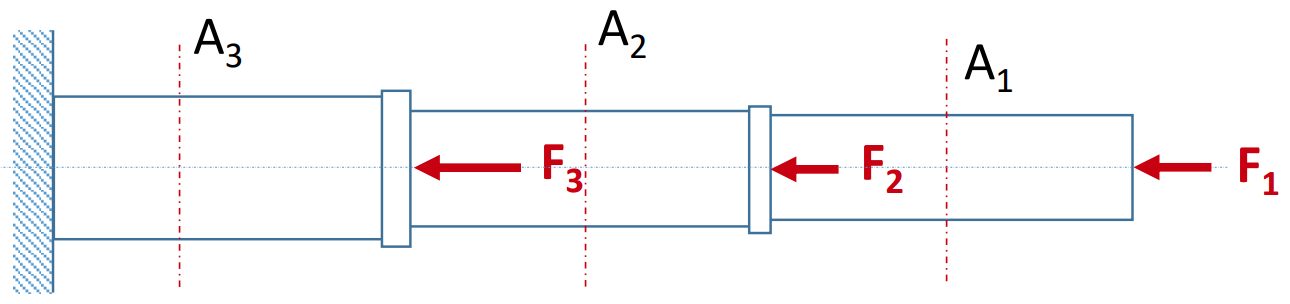
\includegraphics[width = 0.48 \linewidth]{fconc-a}
				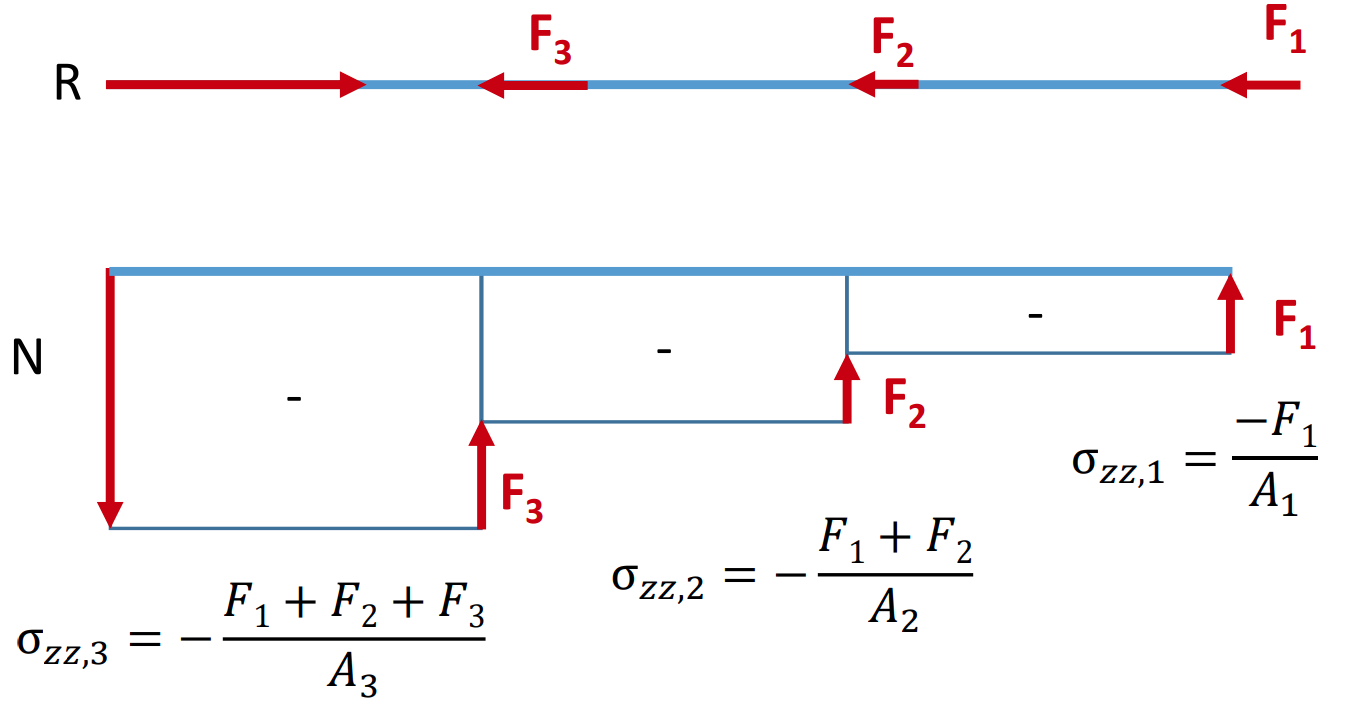
\includegraphics[width = 0.35 \linewidth]{fconc-b}
			\end{center}
			
			\item la teoria di Saint Venant può essere considerata valida anche per \textbf{carichi distribuiti} lungo l'asse della trave (carichi che possono modellare, per esempio, le azioni di volume come la forza peso).
		\end{itemize}
		
		\begin{esempio}{: trave soggetta a carichi distribuiti}
			Si consideri la trave in figura come segue incastrata sulla superficie superiore sul soffitto.
			\begin{center}
				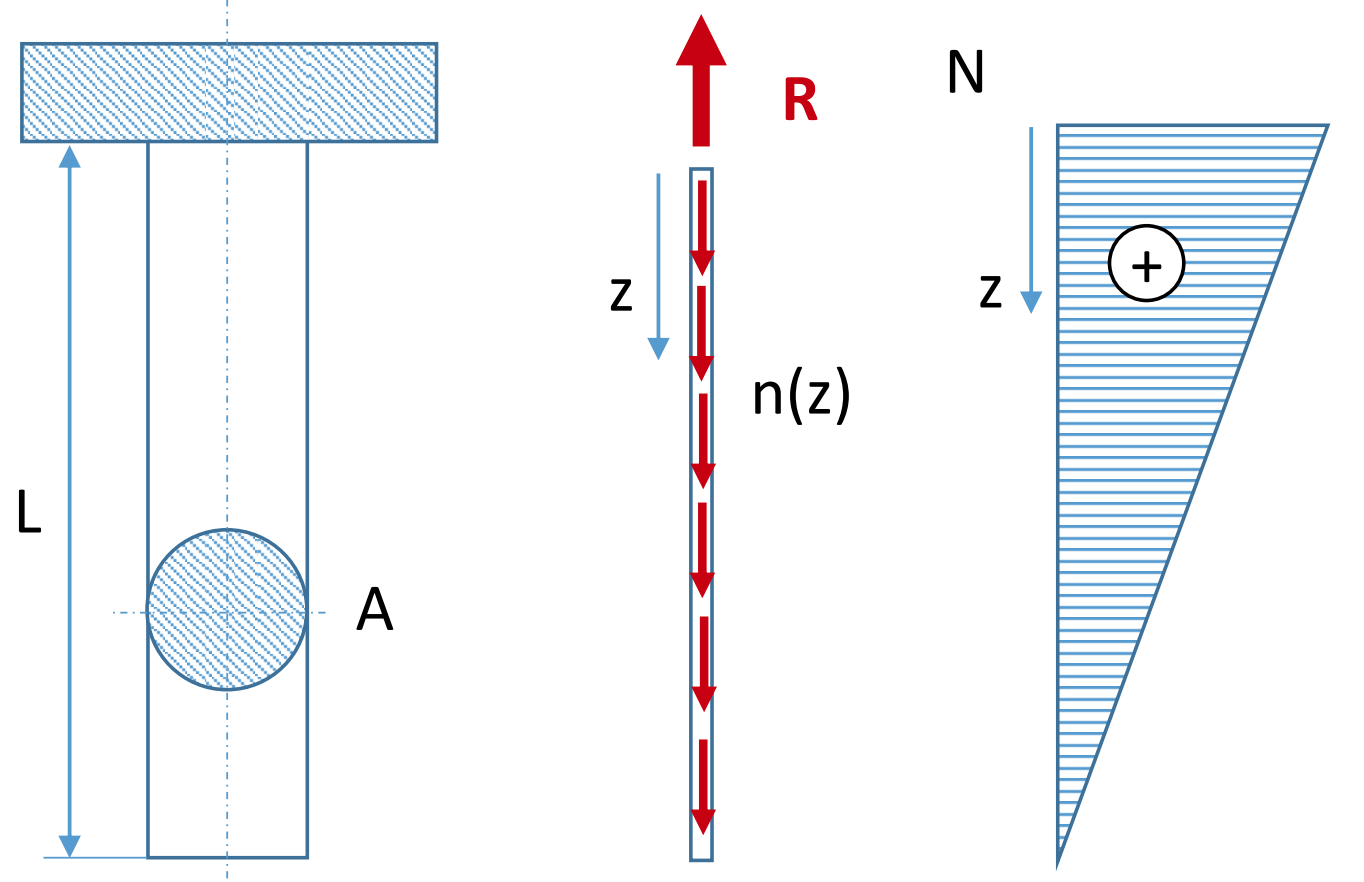
\includegraphics[width=4cm]{az-vol}
			\end{center}
			Della trave è possibile modellare l'azione di volume dovuta al peso come un'azione interna $n(z)$ distribuita di valore $\rho g A$. Per integrazione lungo l'asse è possibile calcolare sia la reazione $R$ in corrispondenza dell'incastro (che rende il sistema statico), sia l'azione interna $N$ in funzione della coordinata $z$ della trave:
			\[ R = \int_0^L n(z)\, dz = \rho g AL \qquad \Rightarrow \quad N(z) = R- \int_0^z n(z')\,dz' = \rho g A\big(L-z\big) = R \left(1 - \frac z L\right) \]
			
			Lo \textbf{stato di tensione} (e conseguentemente di \textbf{deformazione}) si può dunque determinare effettuando il rapporto dell'azione interna $N(z)$ in funzione della posizione nella trave e l'area $A$ della sezione della trave:
			\[ \szz(z) = \frac{N(z)}{A} = \frac RA\left(1- \frac z L\right)  \qquad \Rightarrow \qquad \ezz(z) = \frac{\szz(z)}{E} = \frac R{EA}\left(1- \frac z L\right) \]
			
			La \textbf{variazione di lunghezza} $\Delta L$ può essere determinata sempre tramite integrazione dell'elongazione $\ezz$, con il risultato che
			\[ \Delta L = \int_0^L \ezz(z)  \, dz = \int_0^L \frac{\rho g \big(L-z\big)}{E} \, dz = \frac{\rho gL}{2E} = \frac{RL}{2EA} \]
			L'energia potenziale elastica accumulata dalla trave può essere determinata per integrazione dei potenziali elastici del materiale lineare isotropo lineare:
			\[ U_e = \int_V \psi \, dV \quad \xrightarrow{\psi = \frac{\szz^2}{2E}}\quad \int_0^L \int_A \frac 1 {2E} \frac{R^2}{E^2} \left(1 - \frac z L\right)^2\, dZ\, dz = \frac{R^2L}{6EA} \]
		\end{esempio}

\section{Soluzione di problemi iperstatici}
	\begin{concetto}
		Dato un \textbf{problema} di \textbf{travi vincolate iperstaticamente}, è possibile risolvere lo stesso applicando in maniera sistematica il principio di sovrapposizione degli effetti.
	\end{concetto}
	Per spiegare come risolvere problemi iperstatici verranno mostrati 4 metodi esemplificati nel caso di presenza di sola azione normale $N$, ma i metodi possono essere applicati anche per tutte le altre analisi che verranno mostrate.
	
	In particolare i metodi mostrati si basano tutti sulla risoluzione del problema iperstatico mostrato in figura \ref{fig:sv:traveiperstatica-a}.
	
	\begin{figure}[bht]
		\centering
		\begin{subfigure}{0.48\linewidth}
			\centering
			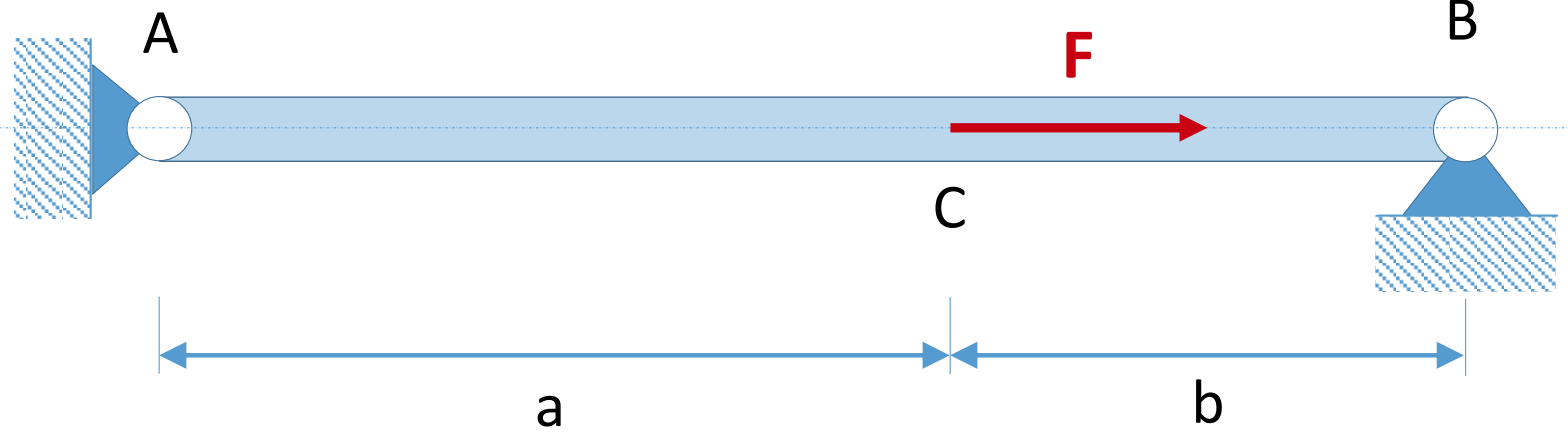
\includegraphics[width=0.9\linewidth]{iperstat-a} \caption{}
		\end{subfigure}
		\begin{subfigure}{0.48\linewidth}
			\centering
			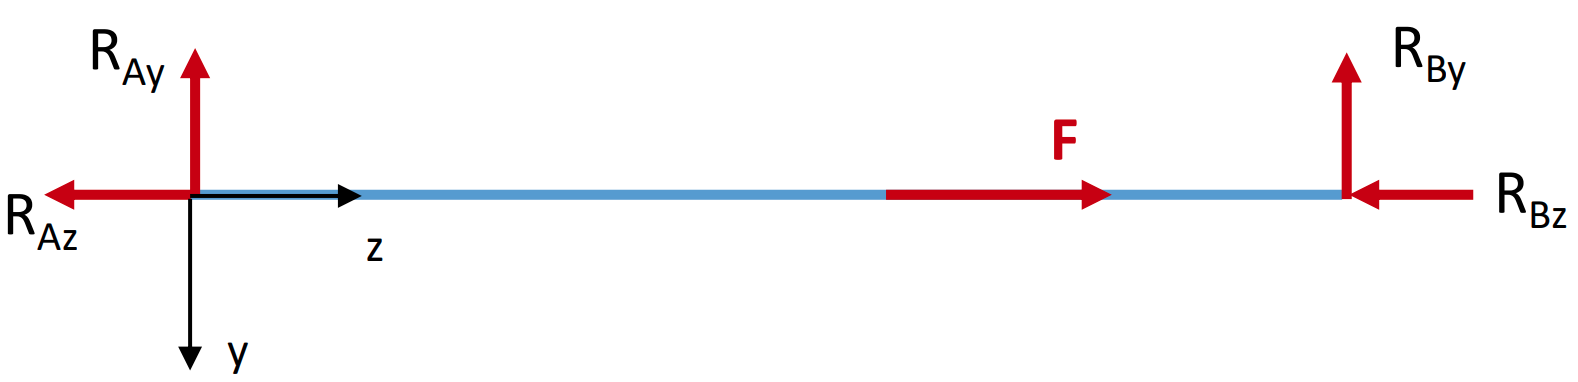
\includegraphics[width=0.9\linewidth]{iperstat-b} \caption{}
		\end{subfigure}
		\caption{trave vincolata iperstaticamente (a) e relativo schema di corpo libero (b).} \label{fig:sv:traveiperstatica-a}
	\end{figure}
	
	\subsection{Metodo delle forze}
		\begin{concetto}
			Il \textbf{metodo delle forze} si basa sulla sostituzione di un vincolo iperstatico con una cosiddetta \textbf{\textit{incognita iperstatica}} $X$; il metodo termina con la risoluzione nelle incognite iperstatiche per rendere congruenti i sistemi ricavati.
		\end{concetto}
		
		Facendo riferimento allo schema in figura \ref{fig:sv:traveiperstatica-a}, è possibile scegliere come incognita iperstatica $X$ la reazione $R_{Bz}$ assiale della trave nella cerniera $B$ e sostituendo la stessa con un pattino (che è libero di traslare).
		
		\figura{7}{0.7}{iperstat-c}{trave dell'esempio in cui viene sostituita la reazione $R_{Bz}$ con l'incognita iperstatica $X$.}{iperstat-c}
		
		
		
		
		
		
		
		
		
		
	